\documentclass{article}

\usepackage{authblk}
\usepackage{amsmath}
\usepackage{tikz}
\usepackage{chngcntr}
\usepackage{wrapfig}
\usepackage{lipsum}
%\usepackage[rightcaption]{sidecap}

\counterwithin{figure}{section}

\author{Aurora Zuoris \\ \normalsize{aurora.zuoris101@alu.ulpgc.es}}
\affil{Universidad de Las Palmas de Gran Canaria}
\title{Matrix multiplication at the speed of light}

\begin{document}

\maketitle

\abstract{
This paper will discuss various methods for implementing matrix multiplication,
along with their advantages and disadvantages for different situations.
Languages explored are Python, Java, C, Rust, and SQL, with methods including
naive, improving cache hits, parallelization, trying to leverage the GPU,
and using a SQL database.
}

\section{Introduction}

Matrix multiplication is becoming increasingly important in the modern world.
Two big examples are machine learning and graph theory, both of which are
becoming more and more important with the rise of big data.
Thus knowing what the best ways to implement matrix multiplication in
various situations is crucial for the future of computing.

In this paper, we will explore two main types of matrices, dense and sparse.
Dense matrices are matrices where most of the values are non-zero,
these are the most common type of matrix, and can be useful for example in deep machine learning,
as they are used to represent the weights and biases of neural networks, such that
a forward pass can be done by multiplying the input by the weight matrix and adding the bias vector,
limiting the speed of the forward pass to the speed of matrix multiplication.
On the other hand, sparse matrices are matrices where most of the values are zero, this can be the case for example
in graphs representing social networks, where most people are not friends with most other people.
Thus sparce matrices only keep track of the non-zero values, and can be stored more efficiently, making it possible
to manipulate matrices that would traditionally be orders of magnitude too large to fit in memory.

\section{Methotology}

The matrix multiplication algorithms will be implemented in various languages, using a plethora
of different optimization techniques, and then benchmarked to see which is the fastest using each
language's timing libraries to get the most accurate results possible.

For brevity and because of time constraints, not all possible combinations of languages and optimization
techniques will be explored, but rather a subset of the most interesting ones.

\subsection{Python}

\subsection{Java}

\subsection{C}

\subsection{C with cache locality}

One way to improve the speed of matrix multiplication is to try to improve cache hits.
The second matrix is looped by rows in the inner loop,
which leads to a lot of cache misses as seen in figure \ref{fig:cache}.
If instead we looped trough the rows, it would lead to more cache hits as in fig \ref{fig:cache2},
but it wouldn't correspond exactly to a matrix multiplication, but it would correspond to $AB^\top$

\begin{wrapfigure}{r}{4cm}
	\begin{minipage}{2cm}
		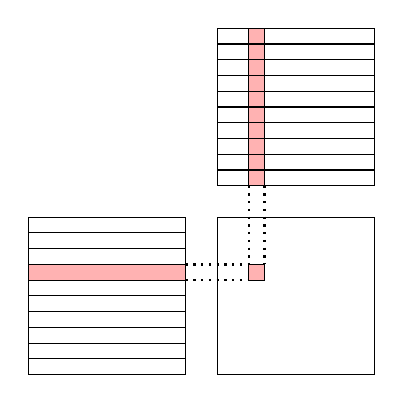
\begin{tikzpicture}[scale=0.2]
			\draw (0,0) rectangle +(10,10);
			\foreach \y in {1, ..., 9}
			{
				\draw (0, \y) -- (10, \y);
			}
			\filldraw[fill=red!30!white] (0, 6) rectangle +(10, 1);
			\draw (12,0) rectangle +(10, 10);
			\draw (12, 12) rectangle +(10, 10);
			\filldraw[fill=red!30!white] (14, 12) rectangle +(1, 10);
			\foreach \y in {1, ..., 9}
			{
				\draw (12, 12+\y) -- +(10, 0);
			}
			\draw[dotted, thick]
				(10, 6) -- (14, 6)
				(10, 7) -- (14, 7)
				(14, 12) -- (14, 7)
				(15, 12) -- (15, 7)
				;
			\draw[fill=red!30!white] (14, 6) rectangle +(1, 1);
		\end{tikzpicture}
\end{minipage}
	\begin{minipage}{2cm}
\caption{
	proper matrix multiplication has a lot of cache misses
}
	\end{minipage}
\label{fig:cache}
\end{wrapfigure}

\lipsum[30]
\lipsum[30]
\lipsum[30]

\begin{wrapfigure}{r}{4cm}
	\begin{minipage}{2cm}
		\centering
		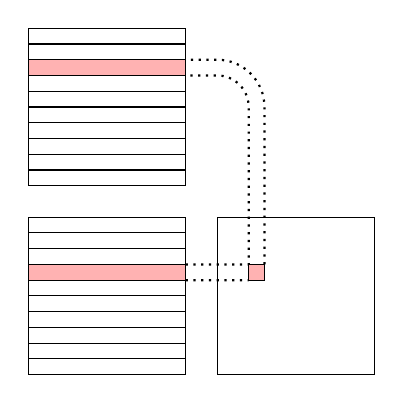
\begin{tikzpicture}[scale=0.2]
			\draw (0,0) rectangle +(10,10);
			\filldraw[fill=red!30!white] (0, 6) rectangle +(10, 1);
			\foreach \y in {1, ..., 9}
			{
				\draw (0, \y) -- (10, \y);
			}
			\draw (12,0) rectangle +(10, 10);
			\draw (0, 12) rectangle +(10, 10);
			\filldraw[fill=red!30!white] (0, 12+7) rectangle +(10, 1);
			\foreach \y in {1, ..., 9}
			{
				\draw (0, 12+\y) -- +(10, 0);
			}
			\draw[dotted, thick]
				(10, 6) -- (14, 6)
				(10, 7) -- (14, 7) -- (14, 17) arc[start angle=0, end angle=90, radius=2] -- (10, 12+7)
				(15, 7) -- (15, 17) arc[start angle=0, end angle=90, radius=3] -- (10, 12+8)
				;
			\draw[fill=red!30!white] (14, 6) rectangle +(1, 1);
		\end{tikzpicture}
	\end{minipage}
	\begin{minipage}{2cm}
	\caption{
		$AB^\top$ has more cache hits
	}
	\end{minipage}
\label{fig:cache2}
\end{wrapfigure}
\subsection{C with parallelization}

\subsection{Rust}

\subsection{Rust with GPU}

\subsection{Python for sparse matrices}

\subsection{Rust for sparse matrices}

\subsection{SQL}

\section{Results}

\section{Conclusion}

\section{Future Work}


\end{document}